\documentclass[12pt, a4paper]{article}

\usepackage{amsmath}
\usepackage{bm}
\usepackage{amsfonts}
\usepackage{amssymb}
\usepackage{graphicx}
\usepackage{float}
\usepackage{listings}
\usepackage{rotating}
\usepackage{verbatim}
\usepackage{tikz}
\pdfgentounicode=1
\pdfmapline{+cyberb@Unicode@  <cyberbit.ttf}

\begin{document}

\title{EvtStatMac}
\date{\today}
\author{Pascal Baillehache}
\maketitle

\tableofcontents

\section{Introduction}

EvtStatMac is a C library to manipulate a event-status machine defined by a finite set of status, a finite set of events (transition from one status to another) and the probabilities for a given event to occur from a given state, and for a given status to be reached after a given event from a given status.\\

The EvtStatMac offers functions to set manually or learn from samples of data the probabilities defining it, to calculate probabilities of all possible combination of event/status given (or not) another event/status, to calculate the probability of a status given a start status and a number of step, to load/save/print its content to a stream, to be cloned, to be normalized/reset, to run a step by step simulation of the phenomenon it modelizes.\\

\section{Definition}

\subsection{Graphic representation of a EvtStatMac}

A EvtStatMac with 2 status ($s_1$, $s_2$) and 2 events ($e_1$, $e_2$) can be represented as follow:\\

\begin{center}
\begin{figure}[H]
\centering
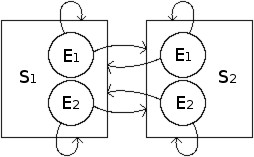
\includegraphics[width=4cm]{./evtstatmac.jpg}
\end{figure}
\end{center}

\subsection{Definition of the behaviour of the EvtStatMac}

The probabilities defining the behaviour of the EvtStatMac are: $P(e|s)$ (the probability for event $e$ to occur when the EvtStatMac is in status $s$) and $P(s'|e,s)$ (the probability to reach status $s'$ when the EvtStatMac is in status $s$ and event $e$ occurs).\\

If the behaviour of the EvtStatMac is learnt from sample data $\{(\bm{s},\bm{e},\bm{s'})\}$ (set of transitions from status $\bm{s}$ to status $\bm{s'}$ through event $\bm{e}$), the values of probabilities above are given by:\\
\begin{equation}
\label{eqnProbEvt}
P_{N_s}(e|s)=
\left\lbrace
\begin{array}{l}
0.0\textrm{, if }N_s = 0\\
\frac{N_{s,e}}{N_s}\textrm{, if }N_s \neq 0\textrm{ and }N_s<N^*\\
\frac{P_{N_s-1}(e|s)+1.0}{N^*+1.0}\textrm{, if }N_s\ge N^*\\
\end{array}
\right.
\end{equation}
and
\begin{equation}
\label{eqnProbTrans}
P_{N_s}(s'|s,e)=
\left\lbrace
\begin{array}{l}
0.0\textrm{, if }N_{s,e} = 0\\
\frac{N_{s,e,s'}}{N_{s,e}}\textrm{, if }N_{s,e} \neq 0\textrm{ and }N_{s,e}<N^*\\
\frac{P_{N_{s,e}-1}(s'|s,e)+1.0}{N^*+1.0}\textrm{, if }N_{s,e}\ge N^*\\
\end{array}
\right.
\end{equation}
where $N_{s}$ is the number of samples where $\bm{s}=s$; $N_{s,e}$ is the number of samples where $\bm{s}=s$ and $\bm{e}=e$; and $N_{s,e,s'}$ is the number of samples where $\bm{s}=s$, $\bm{e}=e$ and $\bm{s'}=s'$; $N^*$ is a maximum number of samples (to avoid overflow problem).\\

If the behaviour of the EvtStatMac is not learnt from sample data, we suppose the probabilities above are set manually by the user.\\

The EvtStatMac is normalized to ensure that:\\
\begin{equation}
\forall{s\in S},\sum_{e\in E}P(e|s)=1.0
\end{equation}
and 
\begin{equation}
\forall{s\in S},\forall{e\in E},P(e|s)\neq0.0\Rightarrow\sum_{s'\in S}P(s'|s,e)=1.0
\end{equation}
where $S$ is the set of possible status, and $E$ is the set of possible events.\\

\subsection{Reminder about probabilities}

We remind that:\\
\begin{equation}
P(A|B)=\frac{P(B|A)P(A)}{P(B)}
\end{equation}\\
\begin{equation}
P(A)=\sum_B\left[P(B)P(A|B)\right]
\end{equation}\\
\begin{equation}
P(A,B)=P(A|B)P(B)
\end{equation}\\
\begin{equation}
P(A,B)=P(B,A)
\end{equation}\\
\begin{equation}
P(A,B,C)=P(A)P(B|A)P(C|A,B)
\end{equation}\\

And we will also use the following equality (proof given in Annex 1):\\
\begin{equation}
P(e,s'|s)=P(s'|s,e)P(e|s)
\end{equation}

\subsection{Probabilities formulas}

Then, from probabilities (\ref{eqnProbEvt}) and (\ref{eqnProbTrans}) we can calculate the other probabilities below.\\

Probability to ends to status $s'$ after $n\in\mathbb{N}^+$ events starting from status $s$:\\
\begin{equation}
P_n(s'|s)=Q_n(s,s')
\end{equation}
where
$$
\left\lbrace
\begin{array}{l}
Q_0(s,s')=
\left\lbrace
\begin{array}{l}
1.0,s=s'\\
0.0,s\neq s'\\
\end{array}
\right.\\
Q_i(s,s')=\sum_{s''\in S}\left[\sum_{e\in E}\left[P(e|s'')P(s'|s'',e)Q_{i-1}(s,s'')\right]\right]
\end{array}
\right.
$$\\

Probability to be in status $s$:\\
\begin{equation}
P(s)=\lim_{i\rightarrow\infty}Q_i(s),i\in\mathbb{N}^+
\end{equation}
where
$$
\left\lbrace
\begin{array}{l}
Q_0(s')=\frac{1.0}{N_s}\\
Q_i(s')=\sum_{s\in S}\left[Q_{i-1}(s)P_1(s'|s)\right]
\end{array}
\right.
$$\\

Probability that event $e$ occurs:\\
\begin{equation}
P(e)=\sum_{s\in S}\left[P(s)P(e|s)\right]
\end{equation}\\

Probability that a transition from status $s$ through event $e$ occurs:\\
\begin{equation}
P(s,e)=P(e|s)P(s)
\end{equation}\\

Probability that a transition from status $s$ to status $s'$ occurs:\\
\begin{equation}
P(s,s')=P_1(s'|s)P(s)
\end{equation}\\

Probability that a transition to status $s'$ through event $e$ occurs:\\
\begin{equation}
\begin{array}{ll}
P(e,s')&=\sum_{s\in S}\left[P(e,s'|s)P(s)\right]\\
&=\sum_{s\in S}\left[P(s'|s,e)P(e|s)P(s)\right]\\
\end{array}
\end{equation}\\

Probability that a transition from status $s$ through event $e$ to status $s'$ occurs:\\
\begin{equation}
P(s,e,s')=P(s)P(e|s)P(s'|s,e)
\end{equation}\\

Probability that a transition started from status $s$ knowing that event $e$ occured:\\
\begin{equation}
P(s|e)=
\left\lbrace
\begin{array}{l}
\frac{P(e|s)P(s)}{P(e)}\textrm{, if }P(e) \neq 0.0\\
0.0\textrm{, if }P(e) = 0.0
\end{array}
\right.
\end{equation}\\

Probability that a transition started from status $s$ knowing that it has ended to status $s'$:\\
\begin{equation}
P(s|s')=
\left\lbrace
\begin{array}{l}
\frac{P_1(s'|s)P(s)}{P(s')}\textrm{, if }P(s') \neq 0.0\\
0.0\textrm{, if }P(s') = 0.0
\end{array}
\right.
\end{equation}\\

Probability that a transition ends to status $s'$ knowing that event $e$ occured:\\
\begin{equation}
P(s'|e)=
\left\lbrace
\begin{array}{l}
\frac{P(e,s')}{P(e)}\textrm{, if }P(e) \neq 0.0\\
0.0\textrm{, if }P(e) = 0.0
\end{array}
\right.
\end{equation}\\

Probability that a transition through event $e$ occured knowing that it ended to status $s'$:\\
\begin{equation}
P(e|s')=
\left\lbrace
\begin{array}{l}
\frac{P(e,s')}{P(s')}\textrm{, if }P(s') \neq 0.0\\
0.0\textrm{, if }P(s') = 0.0
\end{array}
\right.
\end{equation}\\

Probability that a transition started from status $s$ knowing that $e$ occured and ended to status $s'$:\\
\begin{equation}
P(s|e,s')=
\left\lbrace
\begin{array}{l}
\frac{P(s,e,s')}{P(e,s')}\textrm{, if }P(e,s') \neq 0.0\\
0.0\textrm{, if }P(e,s') = 0.0
\end{array}
\right.
\end{equation}\\

Probability that a transition through event $e$ occured knowing that it started from status $s$ and ended to status $s'$:\\
\begin{equation}
P(e|s,s')=
\left\lbrace
\begin{array}{l}
\frac{P(s,e,s')}{P(s,s')}\textrm{, if }P(s,s') \neq 0.0\\
0.0\textrm{, if }P(s,s') = 0.0
\end{array}
\right.
\end{equation}\\

\section{Interface}

\begin{scriptsize}
\begin{ttfamily}
\verbatiminput{../evtstatmac.h}
\end{ttfamily}
\end{scriptsize}

\section{Code}

\begin{scriptsize}
\begin{ttfamily}
\verbatiminput{../evtstatmac.c}
\end{ttfamily}
\end{scriptsize}

\section{Usage}

\subsection{Code}

\begin{scriptsize}
\begin{ttfamily}
\verbatiminput{../evtstatmac_main.c}
\end{ttfamily}
\end{scriptsize}

\subsection{Makefile}

\begin{scriptsize}
\begin{ttfamily}
\verbatiminput{../Makefile}
\end{ttfamily}
\end{scriptsize}

\subsection{Output}

\begin{scriptsize}
\begin{ttfamily}
\begin{lstlisting}
nbStat: 3, nbEvt: 2
Default ESM:
current status: 'stat0'
from status 'stat0'
  by event 'evt0' (0.500000):
    -> status 'stat0' (0.333333)
    -> status 'stat1' (0.333333)
    -> status 'stat2' (0.333333)
  by event 'evt1' (0.500000):
    -> status 'stat0' (0.333333)
    -> status 'stat1' (0.333333)
    -> status 'stat2' (0.333333)
from status 'stat1'
  by event 'evt0' (0.500000):
    -> status 'stat0' (0.333333)
    -> status 'stat1' (0.333333)
    -> status 'stat2' (0.333333)
  by event 'evt1' (0.500000):
    -> status 'stat0' (0.333333)
    -> status 'stat1' (0.333333)
    -> status 'stat2' (0.333333)
from status 'stat2'
  by event 'evt0' (0.500000):
    -> status 'stat0' (0.333333)
    -> status 'stat1' (0.333333)
    -> status 'stat2' (0.333333)
  by event 'evt1' (0.500000):
    -> status 'stat0' (0.333333)
    -> status 'stat1' (0.333333)
    -> status 'stat2' (0.333333)
Random ESM:
current status: 'stat0'
from status 'stat0'
  by event 'evt0' (0.325818):
    -> status 'stat0' (0.430964)
    -> status 'stat1' (0.109718)
    -> status 'stat2' (0.459317)
  by event 'evt1' (0.674182):
    -> status 'stat0' (0.469700)
    -> status 'stat1' (0.107628)
    -> status 'stat2' (0.422671)
from status 'stat1'
  by event 'evt0' (0.382004):
    -> status 'stat0' (0.434699)
    -> status 'stat1' (0.189257)
    -> status 'stat2' (0.376044)
  by event 'evt1' (0.617996):
    -> status 'stat0' (0.407522)
    -> status 'stat1' (0.109232)
    -> status 'stat2' (0.483245)
from status 'stat2'
  by event 'evt0' (0.615099):
    -> status 'stat0' (0.071725)
    -> status 'stat1' (0.465127)
    -> status 'stat2' (0.463149)
  by event 'evt1' (0.384901):
    -> status 'stat0' (0.456197)
    -> status 'stat1' (0.391280)
    -> status 'stat2' (0.152523)
Run few steps:
0: stat0->evt1->stat2
1: stat2->evt1->stat0
2: stat0->evt1->stat2
3: stat2->evt0->stat2
4: stat2->evt0->stat1
Reinit and run few steps:
0: stat0->evt1->stat0
1: stat0->evt1->stat2
2: stat2->evt0->stat2
3: stat2->evt0->stat2
4: stat2->evt1->stat0
Create sample data from ESM
Create another ESM
Learn its behaviour from sample data
Save the learnt ESM to ESM.txt
Load ESM.txt into another ESM
Check the saved and loaded ESMs
Loaded ESM matches original one
Cloned ESM matches original one
Compare all probabilities
Calculated / sample statistics, check precision: 0.000100
P(evt:evt0|from:stat0) = 0.3253 / 0.3253 OK
P(evt:evt0|from:stat1) = 0.3811 / 0.3811 OK
P(evt:evt0|from:stat2) = 0.6157 / 0.6157 OK
P(evt:evt1|from:stat0) = 0.6747 / 0.6747 OK
P(evt:evt1|from:stat1) = 0.6189 / 0.6189 OK
P(evt:evt1|from:stat2) = 0.3843 / 0.3843 OK
P(to:stat0|from:stat0,evt:evt0) = 0.4291 / 0.4291 OK
P(to:stat0|from:stat0,evt:evt1) = 0.4689 / 0.4689 OK
P(to:stat0|from:stat1,evt:evt0) = 0.4313 / 0.4313 OK
P(to:stat0|from:stat1,evt:evt1) = 0.4090 / 0.4090 OK
P(to:stat0|from:stat2,evt:evt0) = 0.0726 / 0.0726 OK
P(to:stat0|from:stat2,evt:evt1) = 0.4545 / 0.4545 OK
P(to:stat1|from:stat0,evt:evt0) = 0.1104 / 0.1104 OK
P(to:stat1|from:stat0,evt:evt1) = 0.1076 / 0.1076 OK
P(to:stat1|from:stat1,evt:evt0) = 0.1911 / 0.1911 OK
P(to:stat1|from:stat1,evt:evt1) = 0.1082 / 0.1082 OK
P(to:stat1|from:stat2,evt:evt0) = 0.4632 / 0.4632 OK
P(to:stat1|from:stat2,evt:evt1) = 0.3917 / 0.3917 OK
P(to:stat2|from:stat0,evt:evt0) = 0.4605 / 0.4605 OK
P(to:stat2|from:stat0,evt:evt1) = 0.4234 / 0.4234 OK
P(to:stat2|from:stat1,evt:evt0) = 0.3776 / 0.3776 OK
P(to:stat2|from:stat1,evt:evt1) = 0.4828 / 0.4828 OK
P(to:stat2|from:stat2,evt:evt0) = 0.4643 / 0.4643 OK
P(to:stat2|from:stat2,evt:evt1) = 0.1538 / 0.1538 OK
P1(to:stat0|from:stat0) = 0.4560 / 0.4560 OK
P1(to:stat0|from:stat1) = 0.4175 / 0.4175 OK
P1(to:stat0|from:stat2) = 0.2193 / 0.2193 OK
P1(to:stat1|from:stat0) = 0.1085 / 0.1085 OK
P1(to:stat1|from:stat1) = 0.1398 / 0.1398 OK
P1(to:stat1|from:stat2) = 0.4357 / 0.4357 OK
P1(to:stat2|from:stat0) = 0.4355 / 0.4355 OK
P1(to:stat2|from:stat1) = 0.4427 / 0.4427 OK
P1(to:stat2|from:stat2) = 0.3450 / 0.3450 OK
P(stat0) = 0.3516 / 0.3516 OK
P(stat1) = 0.2475 / 0.2475 OK
P(stat2) = 0.4010 / 0.4010 OK
P(evt0) = 0.4556 / 0.4556 OK
P(evt1) = 0.5444 / 0.5444 OK
P(from:stat0, evt:evt0) = 0.1144 / 0.1144 OK
P(from:stat0, evt:evt1) = 0.2372 / 0.2372 OK
P(from:stat1, evt:evt0) = 0.0943 / 0.0943 OK
P(from:stat1, evt:evt1) = 0.1532 / 0.1532 OK
P(from:stat2, evt:evt0) = 0.2469 / 0.2469 OK
P(from:stat2, evt:evt1) = 0.1541 / 0.1541 OK
P(from:stat0, to:stat0) = 0.1603 / 0.1603 OK
P(from:stat0, to:stat1) = 0.0382 / 0.0382 OK
P(from:stat0, to:stat2) = 0.1531 / 0.1531 OK
P(from:stat1, to:stat0) = 0.1033 / 0.1033 OK
P(from:stat1, to:stat1) = 0.0346 / 0.0346 OK
P(from:stat1, to:stat2) = 0.1095 / 0.1095 OK
P(from:stat2, to:stat0) = 0.0879 / 0.0879 OK
P(from:stat2, to:stat1) = 0.1747 / 0.1747 OK
P(from:stat2, to:stat2) = 0.1383 / 0.1383 OK
P(evt:evt0, to:stat0) = 0.1077 / 0.1077 OK
P(evt:evt0, to:stat1) = 0.1450 / 0.1450 OK
P(evt:evt0, to:stat2) = 0.2029 / 0.2029 OK
P(evt:evt1, to:stat0) = 0.2439 / 0.2439 OK
P(evt:evt1, to:stat1) = 0.1025 / 0.1025 OK
P(evt:evt1, to:stat2) = 0.1981 / 0.1981 OK
P(from:stat0, evt:evt0, to:stat0) = 0.0491 / 0.0491 OK
P(from:stat0, evt:evt0, to:stat1) = 0.0126 / 0.0126 OK
P(from:stat0, evt:evt0, to:stat2) = 0.0527 / 0.0527 OK
P(from:stat0, evt:evt1, to:stat0) = 0.1112 / 0.1112 OK
P(from:stat0, evt:evt1, to:stat1) = 0.0255 / 0.0255 OK
P(from:stat0, evt:evt1, to:stat2) = 0.1004 / 0.1004 OK
P(from:stat1, evt:evt0, to:stat0) = 0.0407 / 0.0407 OK
P(from:stat1, evt:evt0, to:stat1) = 0.0180 / 0.0180 OK
P(from:stat1, evt:evt0, to:stat2) = 0.0356 / 0.0356 OK
P(from:stat1, evt:evt1, to:stat0) = 0.0626 / 0.0626 OK
P(from:stat1, evt:evt1, to:stat1) = 0.0166 / 0.0166 OK
P(from:stat1, evt:evt1, to:stat2) = 0.0739 / 0.0739 OK
P(from:stat2, evt:evt0, to:stat0) = 0.0179 / 0.0179 OK
P(from:stat2, evt:evt0, to:stat1) = 0.1143 / 0.1143 OK
P(from:stat2, evt:evt0, to:stat2) = 0.1146 / 0.1146 OK
P(from:stat2, evt:evt1, to:stat0) = 0.0700 / 0.0700 OK
P(from:stat2, evt:evt1, to:stat1) = 0.0604 / 0.0604 OK
P(from:stat2, evt:evt1, to:stat2) = 0.0237 / 0.0237 OK
P(from:stat0|evt:evt0) = 0.2511 / 0.2511 OK
P(from:stat0|evt:evt1) = 0.4356 / 0.4356 OK
P(from:stat1|evt:evt0) = 0.2070 / 0.2070 OK
P(from:stat1|evt:evt1) = 0.2813 / 0.2813 OK
P(from:stat2|evt:evt0) = 0.5419 / 0.5419 OK
P(from:stat2|evt:evt1) = 0.2830 / 0.2830 OK
P(from:stat0|to:stat0) = 0.4560 / 0.4560 OK
P(from:stat0|to:stat1) = 0.1542 / 0.1542 OK
P(from:stat0|to:stat2) = 0.3818 / 0.3818 OK
P(from:stat1|to:stat0) = 0.2939 / 0.2939 OK
P(from:stat1|to:stat1) = 0.1398 / 0.1398 OK
P(from:stat1|to:stat2) = 0.2732 / 0.2732 OK
P(from:stat2|to:stat0) = 0.2502 / 0.2502 OK
P(from:stat2|to:stat1) = 0.7060 / 0.7060 OK
P(from:stat2|to:stat2) = 0.3450 / 0.3450 OK
P(to:evt0|evt:stat0) = 0.2364 / 0.2364 OK
P(to:evt1|evt:stat0) = 0.4480 / 0.4480 OK
P(to:evt0|evt:stat1) = 0.3183 / 0.3183 OK
P(to:evt1|evt:stat1) = 0.1882 / 0.1882 OK
P(to:evt0|evt:stat2) = 0.4454 / 0.4454 OK
P(to:evt1|evt:stat2) = 0.3638 / 0.3638 OK
P(evt:stat0|to:evt0) = 0.3063 / 0.3063 OK
P(evt:stat1|to:evt0) = 0.5859 / 0.5859 OK
P(evt:stat2|to:evt0) = 0.5060 / 0.5060 OK
P(evt:stat0|to:evt1) = 0.6937 / 0.6937 OK
P(evt:stat1|to:evt1) = 0.4141 / 0.4141 OK
P(evt:stat2|to:evt1) = 0.4940 / 0.4940 OK
P(from:stat0|evt:evt0, to:stat0) = 0.4559 / 0.4559 OK
P(from:stat0|evt:evt0, to:stat1) = 0.0871 / 0.0871 OK
P(from:stat0|evt:evt0, to:stat2) = 0.2596 / 0.2596 OK
P(from:stat0|evt:evt1, to:stat0) = 0.4560 / 0.4560 OK
P(from:stat0|evt:evt1, to:stat1) = 0.2492 / 0.2492 OK
P(from:stat0|evt:evt1, to:stat2) = 0.5070 / 0.5070 OK
P(from:stat1|evt:evt0, to:stat0) = 0.3777 / 0.3777 OK
P(from:stat1|evt:evt0, to:stat1) = 0.1243 / 0.1243 OK
P(from:stat1|evt:evt0, to:stat2) = 0.1755 / 0.1755 OK
P(from:stat1|evt:evt1, to:stat0) = 0.2568 / 0.2568 OK
P(from:stat1|evt:evt1, to:stat1) = 0.1618 / 0.1618 OK
P(from:stat1|evt:evt1, to:stat2) = 0.3733 / 0.3733 OK
P(from:stat2|evt:evt0, to:stat0) = 0.1664 / 0.1664 OK
P(from:stat2|evt:evt0, to:stat1) = 0.7886 / 0.7886 OK
P(from:stat2|evt:evt0, to:stat2) = 0.5649 / 0.5649 OK
P(from:stat2|evt:evt1, to:stat0) = 0.2871 / 0.2871 OK
P(from:stat2|evt:evt1, to:stat1) = 0.5891 / 0.5891 OK
P(from:stat2|evt:evt1, to:stat2) = 0.1197 / 0.1197 OK
P(evt:evt0|from:stat0, to:stat0) = 0.3062 / 0.3062 OK
P(evt:evt0|from:stat0, to:stat1) = 0.3309 / 0.3309 OK
P(evt:evt0|from:stat0, to:stat2) = 0.3440 / 0.3440 OK
P(evt:evt0|from:stat1, to:stat0) = 0.3937 / 0.3937 OK
P(evt:evt0|from:stat1, to:stat1) = 0.5209 / 0.5209 OK
P(evt:evt0|from:stat1, to:stat2) = 0.3250 / 0.3250 OK
P(evt:evt0|from:stat2, to:stat0) = 0.2037 / 0.2037 OK
P(evt:evt0|from:stat2, to:stat1) = 0.6545 / 0.6545 OK
P(evt:evt0|from:stat2, to:stat2) = 0.8286 / 0.8286 OK
P(evt:evt1|from:stat0, to:stat0) = 0.6938 / 0.6938 OK
P(evt:evt1|from:stat0, to:stat1) = 0.6691 / 0.6691 OK
P(evt:evt1|from:stat0, to:stat2) = 0.6560 / 0.6560 OK
P(evt:evt1|from:stat1, to:stat0) = 0.6063 / 0.6063 OK
P(evt:evt1|from:stat1, to:stat1) = 0.4791 / 0.4791 OK
P(evt:evt1|from:stat1, to:stat2) = 0.6750 / 0.6750 OK
P(evt:evt1|from:stat2, to:stat0) = 0.7963 / 0.7963 OK
P(evt:evt1|from:stat2, to:stat1) = 0.3455 / 0.3455 OK
P(evt:evt1|from:stat2, to:stat2) = 0.1714 / 0.1714 OK
All correct
P2(to:stat0|from:stat0) = 0.3487 / 0.3494 NOK !! 0.000617
P2(to:stat0|from:stat1) = 0.3458 / 0.3463 NOK !! 0.000488
P2(to:stat0|from:stat2) = 0.3576 / 0.3567 NOK !! 0.000841
P2(to:stat1|from:stat0) = 0.2544 / 0.2543 NOK !! 0.000124
P2(to:stat1|from:stat1) = 0.2577 / 0.2571 NOK !! 0.000649
P2(to:stat1|from:stat2) = 0.2350 / 0.2355 NOK !! 0.000508
P2(to:stat2|from:stat0) = 0.3968 / 0.3963 NOK !! 0.000492
P2(to:stat2|from:stat1) = 0.3964 / 0.3966 NOK !! 0.000162
P2(to:stat2|from:stat2) = 0.4074 / 0.4077 NOK !! 0.000333
Not all correct
Nb error: 9
Max error: 0.000841
Avg error: 0.000468
P3(to:stat0|from:stat0) = 0.3523 / 0.3527 NOK !! 0.000403
P3(to:stat0|from:stat1) = 0.3522 / 0.3520 NOK !! 0.000244
P3(to:stat0|from:stat2) = 0.3505 / 0.3503 NOK !! 0.000201
P3(to:stat1|from:stat0) = 0.2463 / 0.2469 NOK !! 0.000598
P3(to:stat1|from:stat1) = 0.2463 / 0.2464 OK
P3(to:stat1|from:stat2) = 0.2492 / 0.2486 NOK !! 0.000564
P3(to:stat2|from:stat0) = 0.4014 / 0.4004 NOK !! 0.001000
P3(to:stat2|from:stat1) = 0.4015 / 0.4016 NOK !! 0.000186
P3(to:stat2|from:stat2) = 0.4003 / 0.4011 NOK !! 0.000764
Not all correct
Nb error: 8
Max error: 0.001000
Avg error: 0.000495
P4(to:stat0|from:stat0) = 0.3515 / 0.3517 NOK !! 0.000155
P4(to:stat0|from:stat1) = 0.3515 / 0.3516 NOK !! 0.000149
P4(to:stat0|from:stat2) = 0.3517 / 0.3514 NOK !! 0.000225
P4(to:stat1|from:stat0) = 0.2476 / 0.2476 OK
P4(to:stat1|from:stat1) = 0.2476 / 0.2481 NOK !! 0.000507
P4(to:stat1|from:stat2) = 0.2473 / 0.2469 NOK !! 0.000354
P4(to:stat2|from:stat0) = 0.4009 / 0.4007 NOK !! 0.000198
P4(to:stat2|from:stat1) = 0.4009 / 0.4003 NOK !! 0.000656
P4(to:stat2|from:stat2) = 0.4010 / 0.4016 NOK !! 0.000579
Not all correct
Nb error: 8
Max error: 0.000656
Avg error: 0.000353
P5(to:stat0|from:stat0) = 0.3516 / 0.3522 NOK !! 0.000601
P5(to:stat0|from:stat1) = 0.3516 / 0.3514 NOK !! 0.000175
P5(to:stat0|from:stat2) = 0.3516 / 0.3511 NOK !! 0.000415
P5(to:stat1|from:stat0) = 0.2475 / 0.2468 NOK !! 0.000630
P5(to:stat1|from:stat1) = 0.2475 / 0.2473 NOK !! 0.000133
P5(to:stat1|from:stat2) = 0.2475 / 0.2481 NOK !! 0.000629
P5(to:stat2|from:stat0) = 0.4010 / 0.4010 OK
P5(to:stat2|from:stat1) = 0.4010 / 0.4013 NOK !! 0.000308
P5(to:stat2|from:stat2) = 0.4010 / 0.4007 NOK !! 0.000214
Not all correct
Nb error: 8
Max error: 0.000630
Avg error: 0.000388
P6(to:stat0|from:stat0) = 0.3516 / 0.3511 NOK !! 0.000446
P6(to:stat0|from:stat1) = 0.3516 / 0.3519 NOK !! 0.000363
P6(to:stat0|from:stat2) = 0.3516 / 0.3517 NOK !! 0.000172
P6(to:stat1|from:stat0) = 0.2475 / 0.2470 NOK !! 0.000472
P6(to:stat1|from:stat1) = 0.2475 / 0.2485 NOK !! 0.001048
P6(to:stat1|from:stat2) = 0.2475 / 0.2472 NOK !! 0.000238
P6(to:stat2|from:stat0) = 0.4010 / 0.4019 NOK !! 0.000918
P6(to:stat2|from:stat1) = 0.4010 / 0.3996 NOK !! 0.001411
P6(to:stat2|from:stat2) = 0.4010 / 0.4010 OK
Not all correct
Nb error: 8
Max error: 0.001411
Avg error: 0.000634
\end{lstlisting}
\end{ttfamily}
\end{scriptsize}

\subsection{ESM.txt}

\begin{scriptsize}
\begin{ttfamily}
\verbatiminput{../ESM.txt}
\end{ttfamily}
\end{scriptsize}

\section{Example 1: Haircut}

\subsection{Problem definition}

The problem is as follow: you are behind a person whose face you cannot see, but you see that this person has long hair. You know that there is as many girls and boys in the population, and you know that half of the girls have long hair, while only 10\% of the boys have long hair. You want to know the probability for the person in front of you to be a boy.\\

This problem can be solved with a EvtStatMac as follow. We define 3 status: 'unknown', 'long hair', 'short hair', and 3 events: 'male', 'female', 'next'. It represents the following process: we pick up an 'unknown' person in the population, it happens to be either a 'male', either a 'female' with an hairstyle status either 'short' either 'long', and we move to the 'next' 'unknown' person.\\

\begin{center}
\begin{figure}[H]
\centering
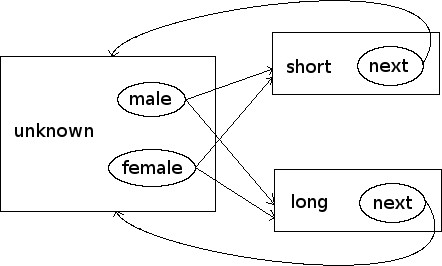
\includegraphics[width=6cm]{./ex1.jpg}
\end{figure}
\end{center}

The behaviour of the EvtStatMac is defined by the following probabilities:\\
$$P(evt:male|from:unknown)=0.5$$
$$P(evt:female|from:unknown)=0.5$$
$$P(evt:next|from:short)=1.0$$
$$P(evt:next|from:long)=1.0$$
$$P(to:short|from:unknown,evt:male)=0.9$$
$$P(to:long|from:unknown,evt:male)=0.1$$
$$P(to:short|from:unknown,evt:female)=0.5$$
$$P(to:long|from:unknown,evt:female)=0.5$$
$$P(to:unknown|from:short,evt:next)=1.0$$
$$P(to:unknown|from:long,evt:next)=1.0$$

The solution of the problem is given by: $$P(evt:male|from:unknown,to:long)$$.\\

\subsection{Code}

\begin{scriptsize}
\begin{ttfamily}
\verbatiminput{../haircut.c}
\end{ttfamily}
\end{scriptsize}

\subsection{Output}

\begin{scriptsize}
\begin{ttfamily}
\begin{lstlisting}
theESM:
current status: 'unknown'
from status 'unknown'
  by event 'Male' (0.500000):
    -> status 'ShortHair' (0.900000)
    -> status 'LongHair' (0.100000)
  by event 'Female' (0.500000):
    -> status 'ShortHair' (0.500000)
    -> status 'LongHair' (0.500000)
from status 'ShortHair'
  by event 'next' (1.000000):
    -> status 'unknown' (1.000000)
from status 'LongHair'
  by event 'next' (1.000000):
    -> status 'unknown' (1.000000)
Probability of Male given Long hair (0.1667): 0.1667
\end{lstlisting}
\end{ttfamily}
\end{scriptsize}

\section{Example 2: Disease}

\subsection{Problem definition}

The problem is as follow: a disease D affects 0.1\% of the population; a medical test for this disease identifies correctly 99\% of sick individual as having the disease and identifies incorrectly 1\% of fine individual as having the disease. We want to know the probability is to have the disease after being test positive once, and after being test positive twice.\\

This problem can be solved with a EvtStatMac as follow. We define 3 status: 'unknown', 'positive', 'negative', and 3 events: 'sick', 'fine', 'next'. It represents the following process: we test an 'unknown' person in the population, it happens to be either a 'fine', or a 'sick' person with a 'positive' or 'negative' result to the test, and we move to the 'next' 'unknown' person.\\

\begin{center}
\begin{figure}[H]
\centering
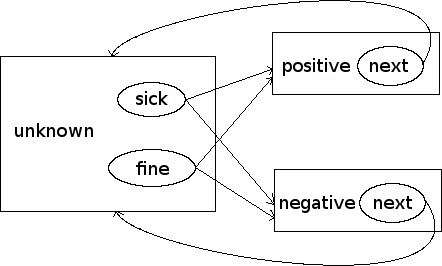
\includegraphics[width=6cm]{./ex2.jpg}
\end{figure}
\end{center}

The behaviour of the EvtStatMac is defined by the following probabilities:\\
$$P(evt:fine|from:unknown)=0.999$$
$$P(evt:sick|from:unknown)=0.001$$
$$P(evt:next|from:positive)=1.0$$
$$P(evt:next|from:negative)=1.0$$
$$P(to:positive|from:unknown,evt:fine)=0.01$$
$$P(to:negative|from:unknown,evt:fine)=0.99$$
$$P(to:positive|from:unknown,evt:sick)=0.99$$
$$P(to:negative|from:unknown,evt:sick)=0.01$$
$$P(to:unknown|from:short,evt:next)=1.0$$
$$P(to:unknown|from:long,evt:next)=1.0$$

The solution of the problem is given by: $$P(evt:sick|from:unknown,to:positive)$$ after the first positive test, then the probability $P(evt:sick|from:unknown)$ is updated with the previous result and the same probability is calculated again for the solution of the problem after the second positive test.\\

\subsection{Code}

\begin{scriptsize}
\begin{ttfamily}
\verbatiminput{../disease.c}
\end{ttfamily}
\end{scriptsize}

\subsection{Output}

\begin{scriptsize}
\begin{ttfamily}
\begin{lstlisting}
theESM:
current status: 'unknown'
from status 'unknown'
  by event 'SickIndividual' (0.001000):
    -> status 'Positive' (0.990000)
    -> status 'Negative' (0.010000)
  by event 'FineIndividual' (0.999000):
    -> status 'Positive' (0.010000)
    -> status 'Negative' (0.990000)
from status 'Positive'
  by event 'next' (1.000000):
    -> status 'unknown' (1.000000)
from status 'Negative'
  by event 'next' (1.000000):
    -> status 'unknown' (1.000000)
Prob of Sick individual given one Positive (0.0902): 0.0902
Update prob of Sick with previous prob
theESM updated:
current status: 'unknown'
from status 'unknown'
  by event 'SickIndividual' (0.090164):
    -> status 'Positive' (0.990000)
    -> status 'Negative' (0.010000)
  by event 'FineIndividual' (0.909836):
    -> status 'Positive' (0.010000)
    -> status 'Negative' (0.990000)
from status 'Positive'
  by event 'next' (1.000000):
    -> status 'unknown' (1.000000)
from status 'Negative'
  by event 'next' (1.000000):
    -> status 'unknown' (1.000000)
Prob of Sick individual given two Positive (0.9075): 0.9075
\end{lstlisting}
\end{ttfamily}
\end{scriptsize}

\section{Example 3: Flu epidemic}

\subsection{Problem definition}

The problem is as follow: you are in charge of some kind of medical institution treating patients of the flu and you must manage resources in prevision of the next epidemic. The epidemic are classified into 12 categories depending on the number of person having the flu in a week. You have records of the category of epidemic of the last 12 years for each week of these year. You need to run simulation of epidemics for training, and forecast the probabilities of categories of current epidemic 3 weeks in advance to get prepared to trigger a special epidemic plan in certain condition.\\

This problem can be solved with a EvtStatMac as follow. We define as many status as there are categories, and as many events as there are weeks. It represents the following process: The EvtStatMac current status is the category of current epidemic from which the event corresponding to 'moving to next week' changes the status to the category of the epidemic at the following week.\\

The behaviour of the EvtStatMac is learnt from real data for flu epidemic in France from 2003 to 2015 ("Data Source: Google Flu Trends (http://www.google.org/flutrends)"). Category $c$ is defined as $c*100\le n<(c+1)*100$ where $n$ is the number of people having the flu during a given week.\\

Simulation can be run by using the {\ttfamily ESMStep()} function, and forecast for outbreak can be calculated with {\ttfamily ESMGetPToGivFrom()}.\\

\subsection{Code}

\begin{scriptsize}
\begin{ttfamily}
\verbatiminput{../epidemic.c}
\end{ttfamily}
\end{scriptsize}

\subsection{Output}

\begin{scriptsize}
\begin{ttfamily}
\begin{lstlisting}
Learning from epidemic data
Artificial data series (week/category):
1/Cat 7, 2/Cat 7, 3/Cat 7, 4/Cat 7, 5/Cat 8, 6/Cat 9, 7/Cat 8, 8/Cat 8, 
9/Cat 8, 10/Cat 7, 11/Cat 7, 12/Cat 6, 13/Cat 6, 14/Cat 5, 15/Cat 5, 
16/Cat 4, 17/Cat 4, 18/Cat 3, 19/Cat 3, 20/Cat 2, 21/Cat 3, 22/Cat 2, 
23/Cat 2, 24/Cat 2, 25/Cat 2, 26/Cat 2, 27/Cat 1, 28/Cat 1, 29/Cat 1, 
30/Cat 1, 31/Cat 1, 32/Cat 1, 33/Cat 1, 34/Cat 2, 35/Cat 3, 36/Cat 3, 
37/Cat 3, 38/Cat 3, 39/Cat 5, 40/Cat 5, 41/Cat 5, 42/Cat 5, 43/Cat 5, 
44/Cat 5, 45/Cat 5, 46/Cat 5, 47/Cat 5, 48/Cat 5, 49/Cat 6, 50/Cat 6, 
51/Cat 6, 
Example of helping management of epidemic special plan.
Check if (prob of cat. 8+) > 25% in 3 weeks.
At week 48 with a current category of Cat 5, 3 weeks forecast:
  to Cat 5: 0.110
  to Cat 6: 0.527
  to Cat 7: 0.278
  to Cat 8: 0.084
  -> No need to trigger the epidemic plan.
Next week (49) with category unchanged, 3 weeks forecast:
  to Cat 5: 0.131
  to Cat 6: 0.508
  to Cat 7: 0.278
  to Cat 8: 0.083
  -> No need to trigger the epidemic plan.
If the category had been Cat 6:
  to Cat 6: 0.290
  to Cat 7: 0.401
  to Cat 8: 0.309
  -> Need to trigger the epidemic plan.
\end{lstlisting}
\end{ttfamily}
\end{scriptsize}

Graphics of 4 simulations of flu epidemic (real data in blue, simulation in black, weeks in abciss, category in ordinate):\\
\begin{center}
\begin{figure}[H]
\centering
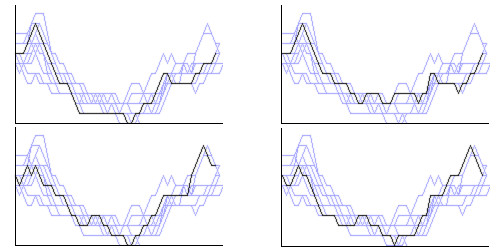
\includegraphics[width=10cm]{./flu.jpg}
\end{figure}
\end{center}

\newpage
\section{Annex 1}
\label{proofA}
Proof of $P(e,s'|s)=P(s'|s,e)P(e|s)$\\
We have:\\
$$
P(s,e,s')=P(s)P(e|s)P(s'|s,e)\\
$$
and\\
$$
P(e,s'|s)=\frac{P(s,e,s')}{P(s)}
$$
then\\
$$
\begin{array}{ll}
P(e,s'|s)&=\frac{P(s'|s,e)P(e|s)P(s)}{P(s)}\\
&=P(s'|s,e)P(e|s)\\
\end{array}
$$

\end{document}

\section{Example 4: Cashier}

\subsection{Code}

\begin{scriptsize}
\begin{ttfamily}
\begin{lstlisting}

\end{lstlisting}
\end{ttfamily}
\end{scriptsize}

\subsection{Makefile}

\begin{scriptsize}
\begin{ttfamily}
\begin{lstlisting}

\end{lstlisting}
\end{ttfamily}
\end{scriptsize}

\subsection{Output}

\begin{scriptsize}
\begin{ttfamily}
\begin{lstlisting}

\end{lstlisting}
\end{ttfamily}
\end{scriptsize}

